\section{Difference-in-differences}

We follow the standard difference-in-differences strategy
\begin{multline}
 \log\left(1 + y_{it}\right) = \sum_{k= \text{1928Q1}}^{\text{1958Q4}} \beta_k \, \text{German}_{i} \cdot \text{YearQuart}_{t}^k + \lambda_t + a_i +  E_i \cdot t \:  + E_i \cdot t^2 \:    + u_{it}
\end{multline}
 %+ \sum_{j= 1}^5 \omega_j \, german_{it} \cdot post_{it - k}    

where $y_{it}$ is number of arrests of people with ethnicity $i$ in year $t$, $\lambda$ is year fixed effect, $a$ is ethnicity fixed effect (both captured by respective dummy variables) and $post$ is a dummy that equals 0 before the year 1933 (exclusive) and 1 after it. The coefficient of interest here is $\delta$. The 5 coefficients $\omega_j$ capture the potential lagged effects (extending from 1934 to 1938), whereas the 3 coefficients capture the lead (anticipatory) effects (from 1930 to 1932) used to test pre-treatment parallel trends.  The $ E_i \cdot t$ term capture the ethnicity specific linear time trends. The inclusion of this term should not significantly  change the coefficients, unless the results are driven by spurious correlation (see \citealt{angrist_mostly_2009}). 

 We apply logarithmic transformation on $y_{it}$ since it better fits the data (more in the results below).  We use $\log\left(1 + y_{it}\right)$ because some observations (although not many) have $y = 0$. As discussed in \citet[p. 193]{wooldridge_introductory_2015},  the percentage change interpretation is usually  closely preserved (except for changes beginning at 0 which are not of interest to us).   

Our identifying assumption is that the number of arrest of Germans after 1933 would go in parallel to arrests of other minorities in the absence shock to German-Soviet relations conditional on our control variables (mainly the ethnicity specific time trends). Although we cannot test this assumption, we can test whether the trends were parallel prior to 1933 (pre-treatment) which could increase our confidence that they were parallel after 1933 too. This can be testing if the coefficients on lead effects ($\gamma_k$) are significantly different from zero.  

As \citet{bertrand_how_2004} show, the usual standard errors  are downward-biased for most DiD regressions since they do not account for the serial correlation within the units of interests (states, countries etc.). A common solution to this problem is to estimate standard errors using robust covariance matrix that allows for clustering (i.e. cluster-robust standard errors). However for small number of groups (generally less than 40), the cluster-robust standard errors are downward-biased and not reliable. \citet[chapter 8]{angrist_mostly_2009} suggest taking the maximum of cluster-robust as a simple rule of thumb to avoid gross misjudgements in precision. More rigorous solutions are cluster bootstrapping \citep{cameron_bootstrap-based_2008, cameron_practitioners_2015} and  using $t$-distribution with $G- K$ degrees of freedom (where $G$ is number of clusters and $K$ number of parameters) rather than the standard Normal distribution \citep{mccaffrey_bias_2002, imbens_robust_2016}. 

Since we have small number of groups we use bell correction ...  

\subsection{Results}

The results of our main specification are presented in the table \ref{dif_table}, in column (1). The estimated coefficients together with their 95\% confidence  from this model are plotted in the figure \ref{fig_did_effets}. We can see that all coefficients for years 1930 to 1932 are statistically insignificant which means that the pre-treatment trends in arrests of German minority were likely parallel to the pre-treatment trends of other minorities which gives us greater  confidence in the validity of our identification strategy. 

The coefficients on all other years are insignificant as well. Only for 1934 (one year lag) is the estimate  significant at 10\% level ($p$-value of 0.08). Since this not reaches even the traditional 5\% significance threshold we are inclined to not reject the null hypothesis or at least to conclude that evidence in favor of the alternative hypothesis (more repressions of Germans due to rise of Hitler) is quite weak.  Furthermore, as we show below the alternative specifications do not increase the significance of the coefficients.
\begin{figure}[h]
\centering
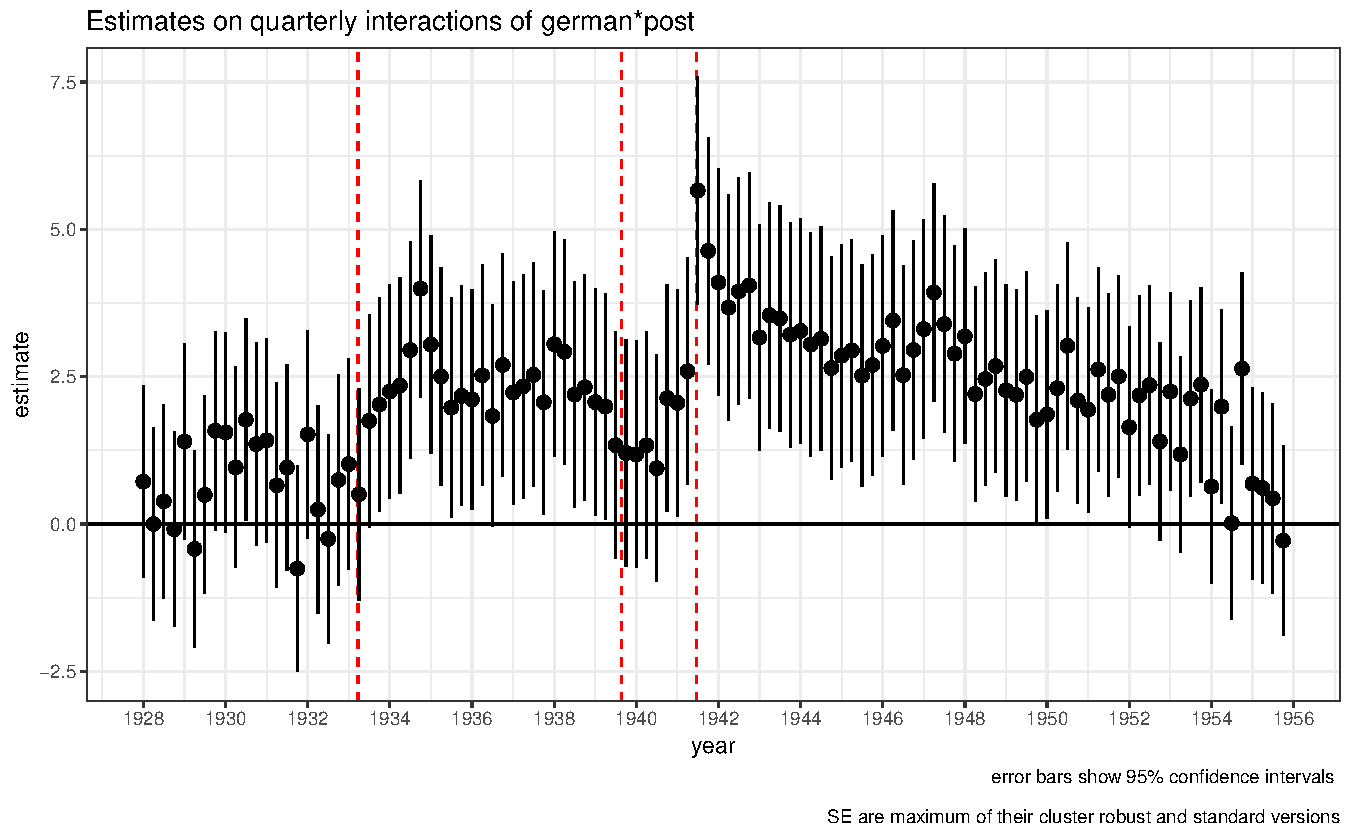
\includegraphics[width=\textwidth]{plots/effects/quarterly/pointrange.pdf}
\caption{Estimates of coefficients on $german \cdot post\_year$}
\label{fig_did_effets}
\end{figure}
%We perform several robustness checks to asses sensitivity of the results to different specifications. First, in our main model (column (1) of table \ref{dif_table}), we included all observations in years 1923 to 1958. But the relationship between Germany and Soviet Union were somewhat more complicated after the World War II. We thus re-estimate the model with only the data from 1923 to 1945. The results (in column (2)) change only little and does not alter our previous conclusions. Second, when we omit the ethnicity specific linear time trends in column (3), we see again that the coefficients are very similar to the original model. Finally, we estimate a specification with number of arrests as a dependent variable (without logarithmic transformation). We can see that this model (shown in column (4)) fits the data rather poorly with  $R^2$ only of 0.428 (compared to 0.890 in the logarithmic specification). 

\section{Synthetic Control Method}
However, the parrarel trends assumption can sometiemes be violated. These issues can be adressed by sythetic control method
\citep{abadie_synthetic_2010, abadie_economic_2003}. We closely follow \citet{abadie_synthetic_2010}.

Let $Y_{it}$ be log of number of arrests of individuals belonging to an ethnic group $i$ at time $t$ with $i = 1$ being German ethnicity.  We
denote $D_{1t}$ as the treatment dummy, i.e. variable that equals 1 if $i = 1$ and $T > \text{1933Q1}$ (Hitler's rise to power) and 0 otherwise. 
Let be $Y_{1t}^N$ be a counterfactual log of number of arrests of Germans in the absence of treatment. SCM assumes a model
\begin{equation}
    Y_{1t} = Y_{1t}^N + \alpha_{1t} \, D_{1t}
\end{equation}
Furthermore, we assume that $Y_{1t}^N$ is given by the following factor model:
\begin{equation}
   Y_{1t}^N = \delta_t + \boldsymbol{\theta}_t \boldsymbol{Z}_i +
   \boldsymbol{\lambda}_t \boldsymbol{\mu}_i + \epsilon_{it}
\end{equation}
where is $\delta_t$ an unknown common factor with constant factor
loadings across units, $\boldsymbol{Z}_i$ is a
$(1 \times r)$ vector of observed time-invariant covariates (unaffected by the treatment),  $\boldsymbol{\theta}_t$ is a $(1 \times r)$ vector of
unknown parameters, $\boldsymbol{\lambda}_t$ is a $(1 \times F)$ vector of unobserved time-varying factors, $\boldsymbol{\mu}_i$ is an $(F \times 1)$ vector of unknown factor loadings
and $\epsilon_{it}$ is the error term with zero mean. 

Notice that for constant  $\boldsymbol{\lambda}_t$ for all $t$ we get the traditional  difference-in-differences model. Unlike difference-in-differences,  the synthetic control method  allows for unit-specific time trends as long as they can be captured by the factor model. 

The synthetic control works by contracting a control group for which the average of its factor loadings $\boldsymbol{\mu}_i$ match the factor loadings of the treated unit  $\boldsymbol{\mu}_1$.

For pre-treatment

\subsection{Results}
We implemented the synthetic control method in R software using the MSCMT package \citep{becker_fast_2018}. The calculated optimal weights of ethnic groups in the synthetic German minority are provided in the table \ref{tab:sc_weights} (ethnic groups with zero weight are not shown). The highest contribution in the synthetic German minority have the Ossetians, Tatars and Pols with weights 0.39, 0.23 and 0.14 respectively. The Greek, Kabaradin, Chechen, Lithuanian and Ukrainian minorities are also partially reflected in the synthetic control although only with very small weights. 
\begin{table}[t]

\caption{\label{tab:sc_weights}Synthetic German minority weights}
\centering
\begin{tabular}{lr}
\toprule
Ethnic group & \$W\$-Weight\\
\midrule
Greek & 0.32\\
Kabardian & 0.09\\
Chuvash & 0.08\\
Moldovan & 0.07\\
Belorussian & 0.06\\
Polish & 0.06\\
Finnish & 0.06\\
Altai & 0.04\\
Armenian & 0.04\\
Georgian & 0.03\\
Ossetian & 0.02\\
Chechen & 0.02\\
Kazakh & 0.02\\
Bashkir & 0.02\\
Jewish & 0.02\\
Ukrainian & 0.01\\
Bulgarian & 0.01\\
Latvian & 0.01\\
Chinese & 0.00\\
\bottomrule
\end{tabular}
\end{table}


Figure \ref{fig_sc_comp_plot} shows the trends in arrests for the German minority and its synthetic control. The synthetic German minority tracks the actual values fairly well except for two large negative shocks to the actual arrests in 1931 and 1932 which the synthetic control does not capture. The trends start to diverge in the second quarter of 1933 with the actual arrests of Germans holding steady but decreasing for synthetic control. 
The gap between the trends for the actual German minority and its synthetic control (shown in figure \ref{fig:sc_placebo_gaps_all}) keeps within the range of 1.25 to 2.5 for most of the post-1933 period. This implies that the rise of Hitler led to about  2\% increase in the arrests of Germans by the NKVD  in the period from 1933 to 1939. This is very similar to the estimates obtained using difference-in-differences. 
%The figure shows increase between 1937 and 1939 (the period of the Great Terror).  
\begin{figure}[h]
\centering
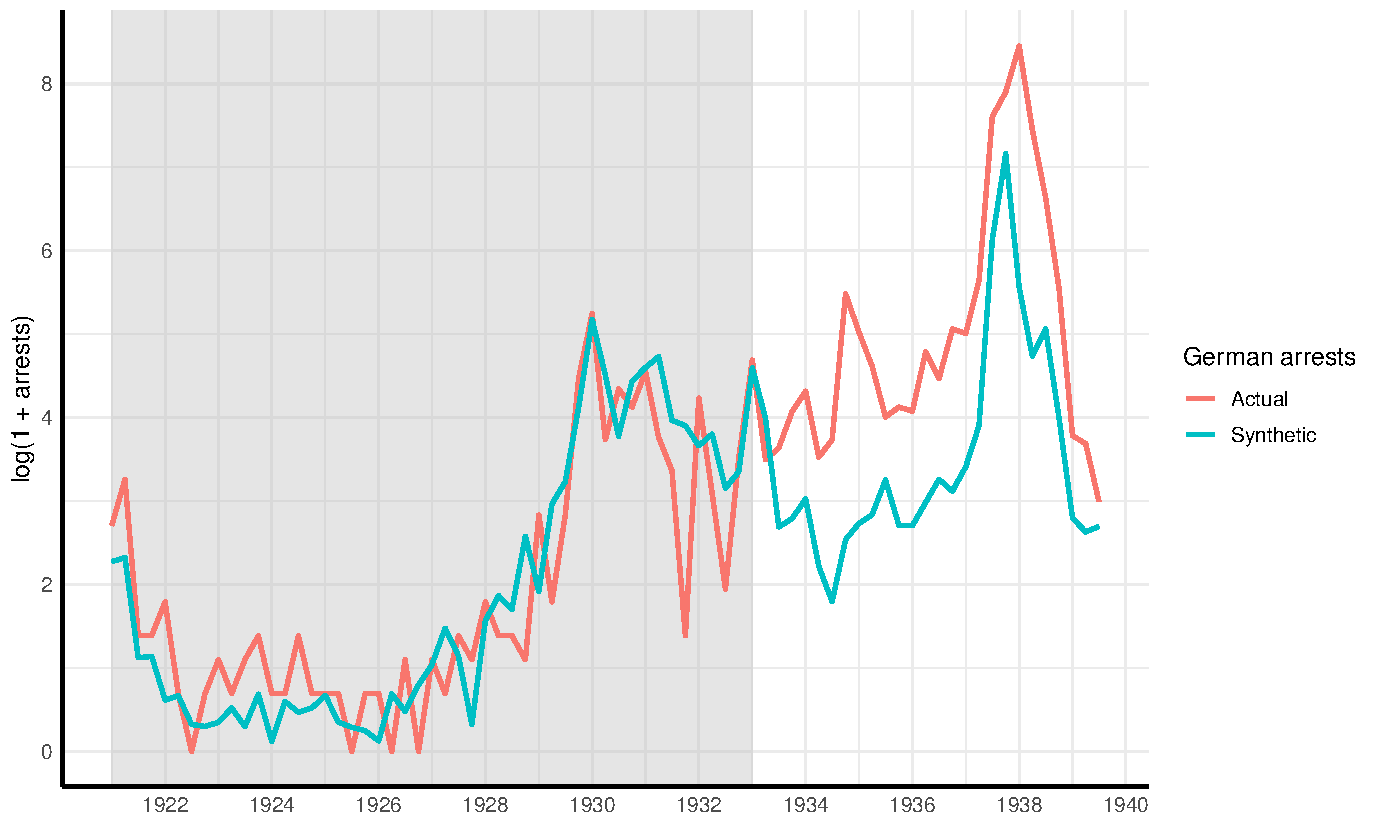
\includegraphics[width=\textwidth]{plots/synthetic_control/until_pact/comparison_plot.pdf}
\caption{Comparison plot}
\label{fig_sc_comp_plot}
\end{figure}


%\subsubsection{Inference}
The synthetic control method, however, by itself does not provide us with any measure of uncertainty of significance. This has been addressed by performing placebo tests \citep{abadie_synthetic_2010}. Synthetic control method is applied iteratively to every ethnicity in the donor pool
%with the same treatment period
as if they were treated. By comparing the gaps from these placebo tests with the gap for the German minority, we can assess the
significance of our results.
Large gaps for arrests of Germans relative to other ethnic groups would suggest that the results are significant since these results would be less likely if there were no treatment effect . 
%The estimated  gaps between the synthetic control and the actual data for every ethnic group is shown in figure \ref{fig:sc_placebo_gaps}. 

Figure \ref{fig:sc_placebo_gaps_all} shows gaps between the synthetic control and the actual trends for Germans together with placebo gaps for all 17 other ethnic groups. The post-treatment gap for German minority is relatively large although not the highest. The figure also highlights that for some ethnic groups the pre-treatment gaps are large too. This indicates that synthetic control of these ethnic groups does not capture the actual pre-treatment trends well. As \citet{abadie_synthetic_2010} note, placebo synthetic controls  with poor pre-treatment fit do not provide good comparison
%are not very helpful for
for estimating rareness of large  post-treatment gap for a treatment with a good pre-treatment fit. They thus recommend excluding excluding placebo groups with substantially higher pre-treatment mean squared prediction error  (MSPE)
%(the average of squared differences between the value of the outcome for synthetic and actual) 
%relatively to the treated group. 
%In our case the pre-treatment MSPE of the German minority is fairly small (0.52). 
%If we exclude minorities with the pre-treatment MSPE
%If we choose the cutoff for exclusion as the MSPE 

%Morever, the pre-treatment MSPE is quite small (0.52) which means that the synthetic German minority captures the actual pre-treatment trends relatively well. However, the pre-treatment MSPE of a few minorities is much larger indicating that no combination of donor ethnic groups fits well their time series. As \citet{abadie_synthetic_2010} note,  if there is poor fit of the synthetic control to the actual trends in the pre-treatment period then its post-treatment gap does not provide good comparison to the well fit ethnic groups. 
%large post-treatment gap would not indicate the presence of an effect but  
Following \citet{abadie_synthetic_2010}  we therefore exclude ethnic groups whose pre-treatment MSPE is 5 times higher then the same measure for German minority. This removes 4 ethnic groups with the worst pre-treatment fit (Tatars, ...). The resulting plot is shown in the figure \ref{fig:sc_placebo_gaps_all_5_times}. The post-1933 gaps in German arrests now stand out more clearly. 

\begin{figure}[hbtp] 
\begin{subfigure}{\textwidth}
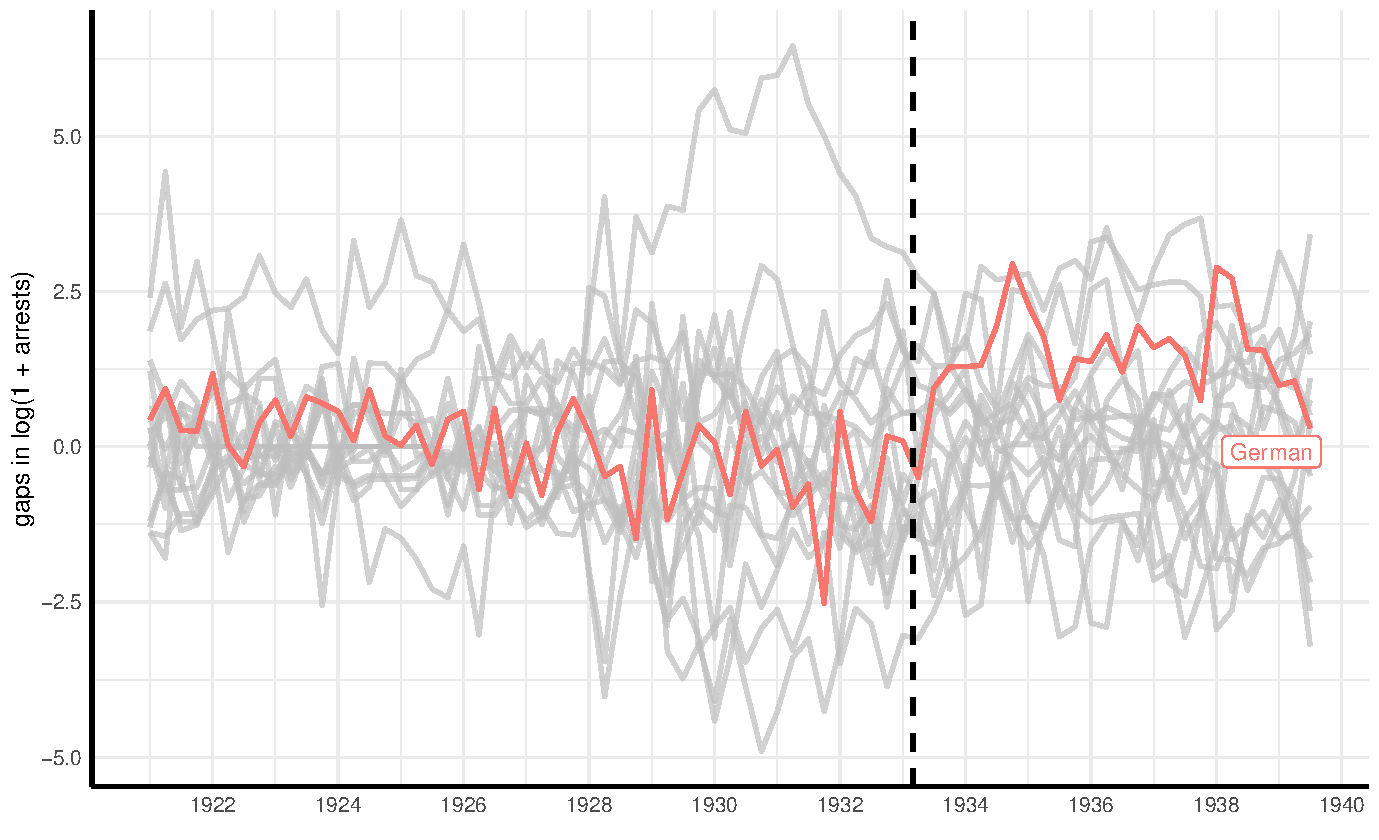
\includegraphics[width=0.9\linewidth]{plots/synthetic_control/until_pact/placebo_highlight_all.pdf}
\caption{All ethnic groups}
\label{fig:sc_placebo_gaps_all}
\end{subfigure}
\begin{subfigure}{\textwidth}
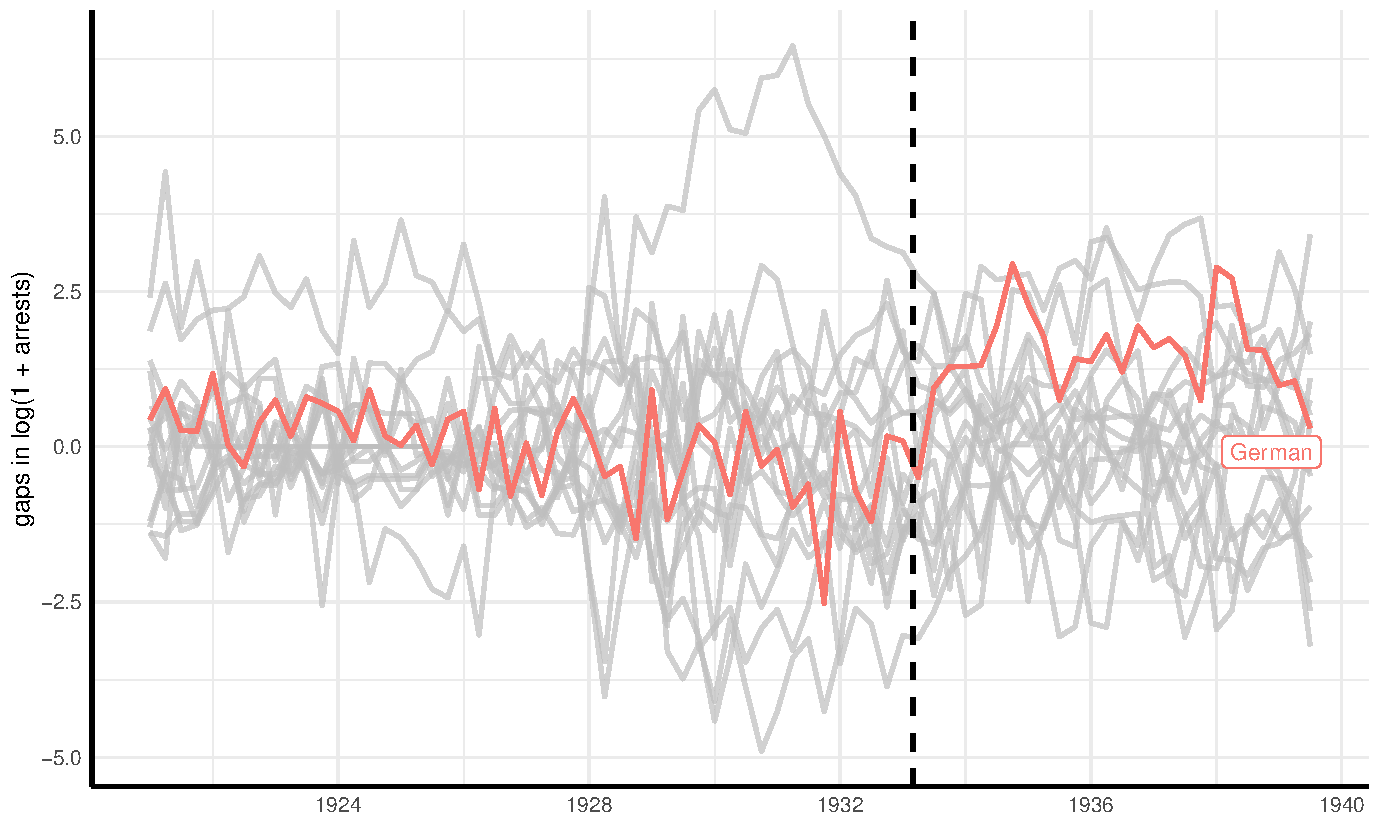
\includegraphics[width=0.9\linewidth]{plots/synthetic_control/until_pact/placebo_highlight_mspe_5_lower.pdf}
\caption{Ethnic groups with pre-treatment MSPE higher than 5 times the MSPE of Germany excluded}
\label{fig:sc_placebo_gaps_all_5_times}
\end{subfigure}
\caption{Gaps between synthetic control and actual values}
\label{fig:sc_placebo_gaps}
\end{figure}

Nevertheless, the choice of any level of the cutoff of pre-treatment MSPE %for exclusion of 
is somewhat arbitrary. Alternative way to asses significance of results may be to compare the ratios of  post/pre-treatment MSPE.  The values of these ratios for all ethnic groups are displayed in the figure \ref{fig:sc_mspe_ratios}. Post/pre-treatment MSPE ratio for the German minority is by far the highest. The probability of obtaining such a result if the is 0. 

%This is shown in  the figure \ref{fig_sc_mspe_hist}
\begin{figure}[h]
\centering
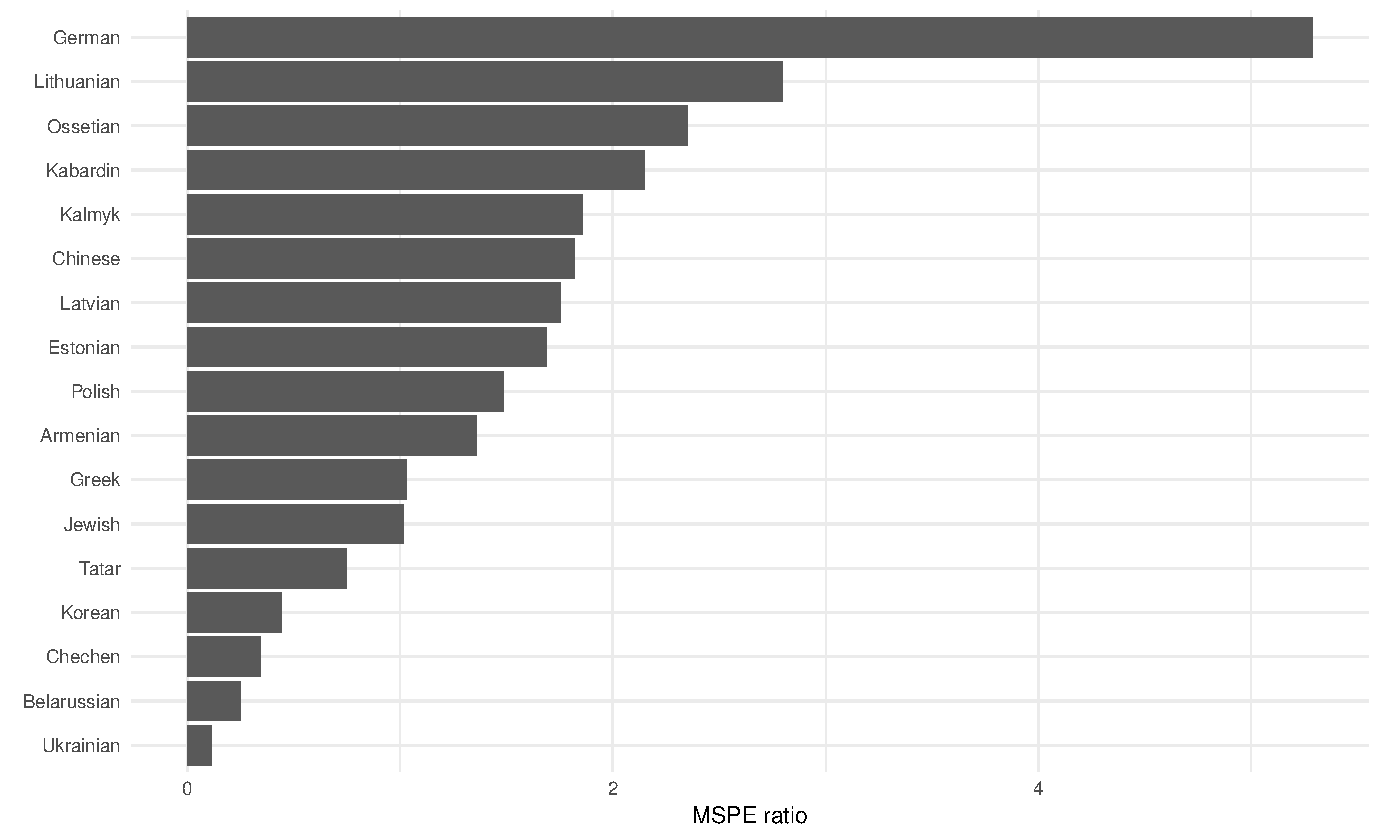
\includegraphics[width=\textwidth]{plots/synthetic_control/mspe_ratios.pdf}
\caption{Ratios of post-treatment MSPE to pre-treatment MSPE}
\label{fig:sc_mspe_ratios}
\end{figure}
%\subsection{Generalized Synthetic Control Method}
%\citet{xu_generalized_2017}